\chapter{Interactive Object Recognition}
\label{chapter:Object Recognition}

\section{Challenges}
As suggested in Chapter \ref{chapter:Introduction} there are many difficulties in feature matching based object recognition systems that mainly stem from view point variance of features, change in lighting conditions, and noisy sensors. In order to establish the underlying cause of difficulty, we implemented an object recognition system that extracts features from live images streamed from a Kinect camera.  It then matches them against features extracted from images in the database. The system can in turn recognize which object is seen in the input image based on the number of matches.  For the rest of this section, ``input image'' refers to the image being streamed from the Kinect camera.

\subsection{Lighting Conditions and Sensor Noise}

During our experiments we noted that when matching between input and database image, many of the features in the input image were flickering even though the object was not moved with respect to the camera. 

To investigate this, an instance of a flickering feature point was identified, and the keypoint location recorded.  Two image patches encompassing the feature point were then saved: one when a positive feature match at this keypoint occurred, and one when no match was found. %Take note that this feature ``patch'' is not exactly what the actual feature extractor used for matching, depending on the feature type, it is purely for visualization.

Figure \ref{fig:patches} shows two pairs of such feature patches taken at two consecutive frames and the difference image between them. Looking at this difference image (see last column in Figure \ref{fig:patches}) it can be clearly seen that there was a significant change in the input image even though nothing was changed in our set-up. In this case, it was found that the feature detector failed to identify an interest point at this location for when no match occurred.  As nothing changed in our set-up, this failure is assumed to be due to difference in lighting and or noise from the sensor.

\begin{figure}
\centering

{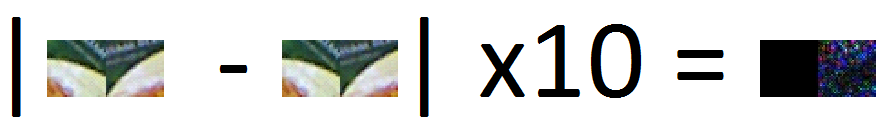
\includegraphics[width=1\columnwidth]{figures/patches.png}}

\caption[Difference between two pairs of images for a stationary object.]{Difference between two pairs of images for a stationary object. The first patch of the pair is the feature patch from the database image. The second patch in the pair is the feature patch from the input image. The second pair shows the image patch in the same location but for a frame where there was no match of this feature.  One of the pairs was subtracted from the other to compute a difference image.  The difference image was then multiplied by a factor of 10. This shows a significant difference between database and input patches. There is no difference in the database image patch because it is the same patch for both pairs.  This indicates the influence that lighting and sensor noise have on the image.}
\label{fig:patches}
\end{figure}

\begin{figure}
\centering
    \begin{tabular}{c}
 

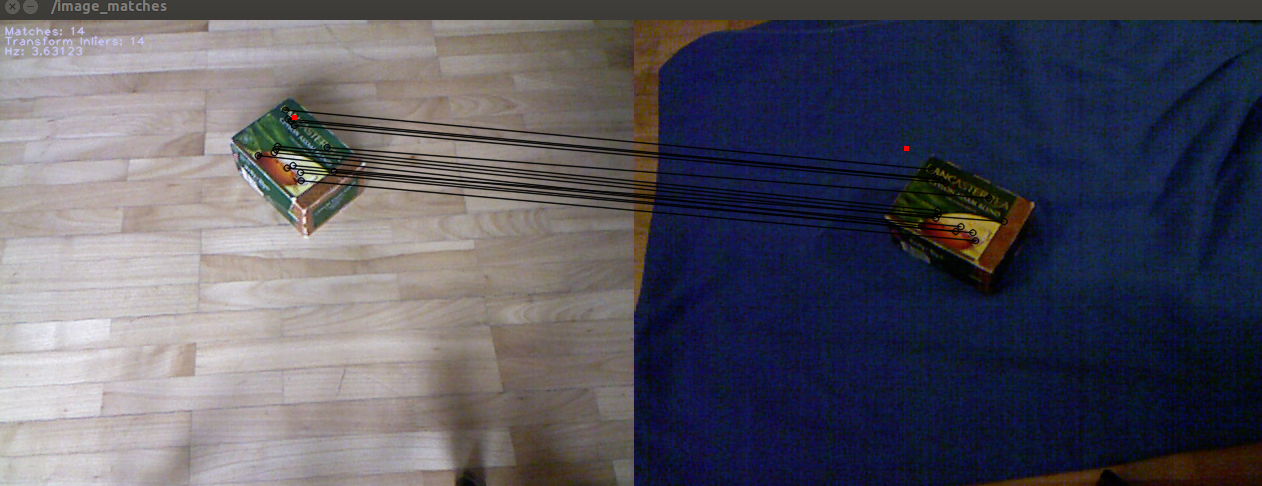
\includegraphics[width=0.7\columnwidth]{figures/sift-gpu-no-rotation.png}\\
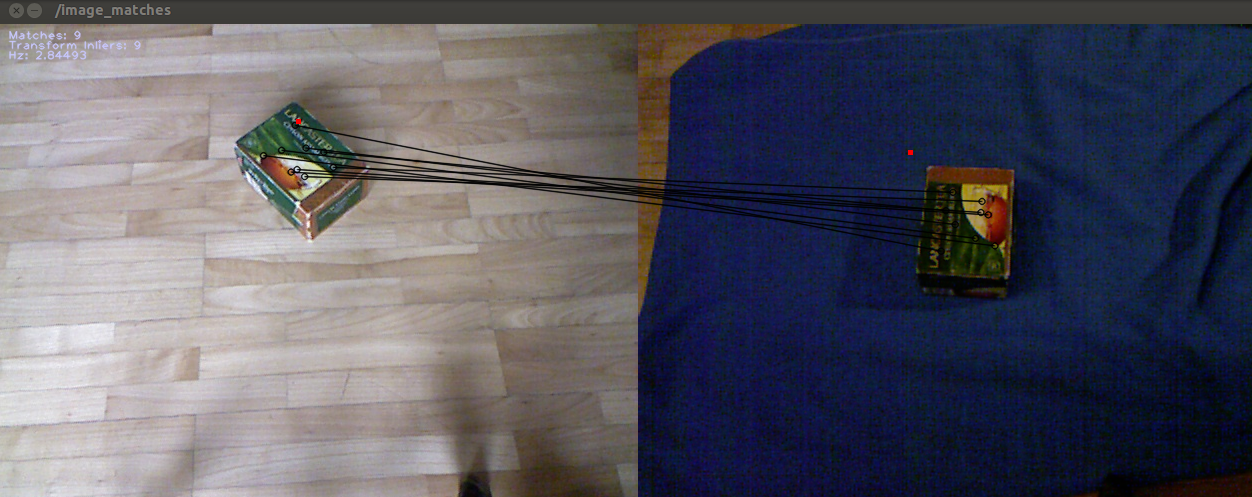
\includegraphics[width=0.7\columnwidth]{figures/siftgpu-rotation.png}\\
    \end{tabular}


\caption[Comparison of two pairs of images being matched using SIFT detector and SIFT descriptor.]{Comparison of two pairs of images being matched using SIFT detector and SIFT descriptor. The upper image shows the object in the original pose and the lower shows the rotated object. It is apparent that the number of feature matches significantly decreases if the object is rotated. }
\label{fig:sift-features}
\end{figure}

\begin{figure}
\centering
    \begin{tabular}{c}
 

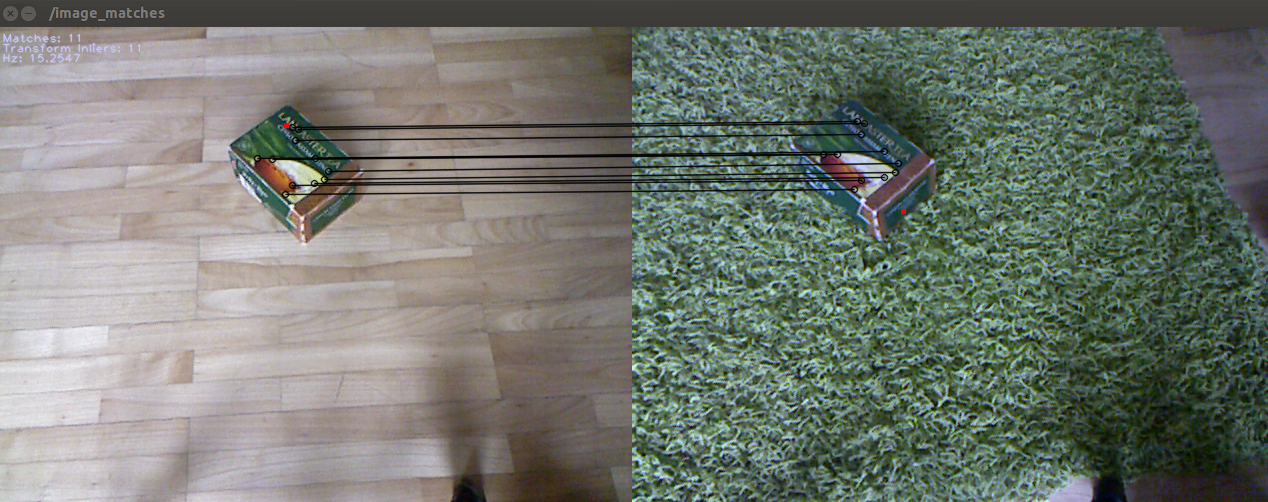
\includegraphics[width=0.7\columnwidth]{figures/freak-no-rotation.png}\\
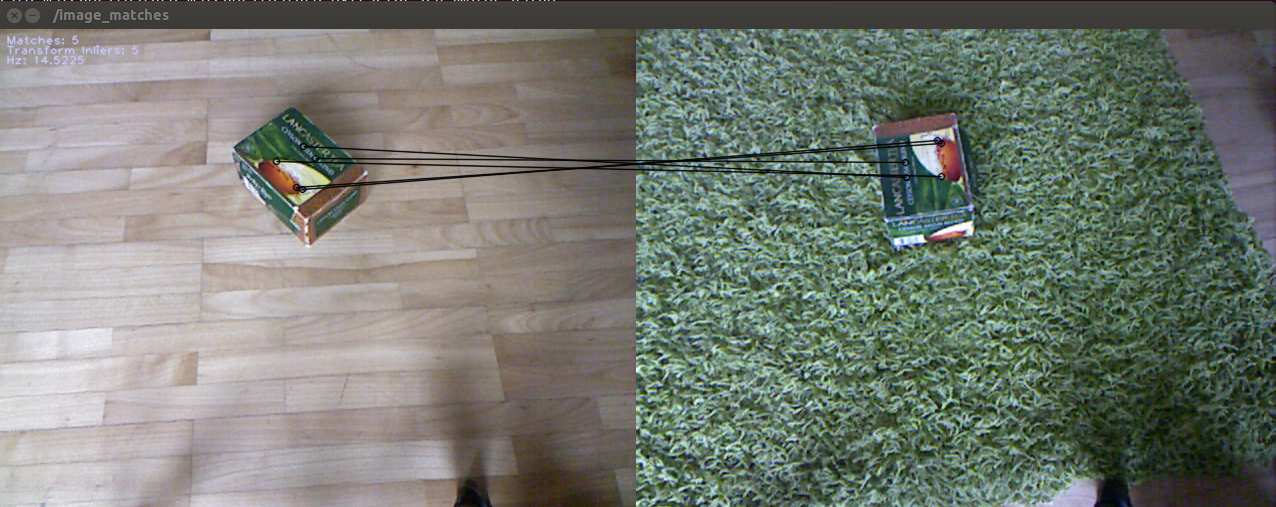
\includegraphics[width=0.7\columnwidth]{figures/freak-rotation.png}\\
    \end{tabular}


\caption[Comparison of two pairs of images being matched using FAST detector and FREAK descriptor.]{Comparison of two pairs of images being matched using FAST detector and FREAK descriptor. The upper image shows the object in the original pose and the lower shows the rotated object. It is apparent that the number of feature matches significantly decreases if the object is rotated. }
\label{fig:freak-features}
\end{figure}

%\begin{figure}
%\centering
%    \begin{tabular}{c}
 

%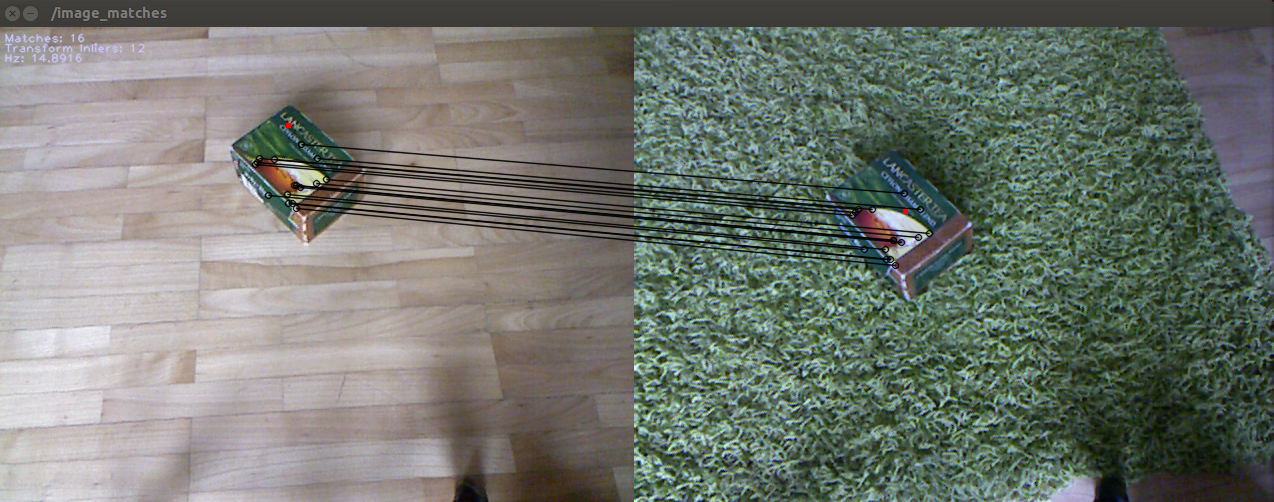
\includegraphics[width=0.7\columnwidth]{figures/brief-no-rotation.png}\\
%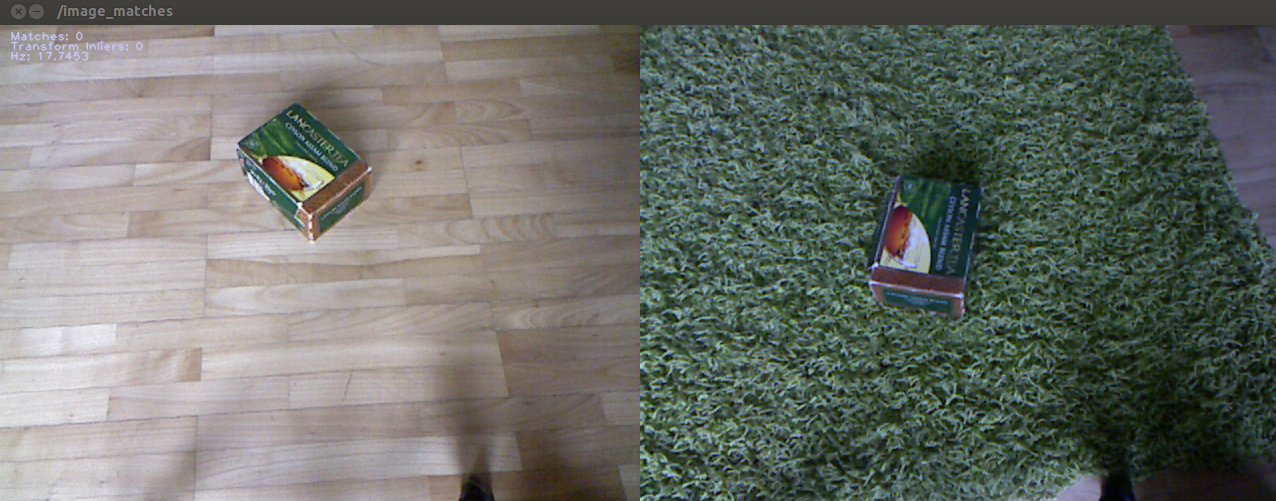
\includegraphics[width=0.7\columnwidth]{figures/brief-rotation.png}\\
%    \end{tabular}


%\caption{Comparison of two pairs of images using FAST detector and BRIEF descriptor. The upper image shows the object in the original pose whereas the lower shows the rotated object. It can be noticed that number of feature matches significantly decreases if the object is rotated. }
%\label{fig:brief-features}
%\end{figure}


\subsection{View-point Variance}

In order to demonstrate the problem of view-point variance of the feature descriptors we compared two input images of the same object.  One was taken in the same pose as it occurs in the database image and another where the object is rotated. We tested these pairs with two different detectors and descriptors to ensure that the problem is not associated with a particular detector-descriptor pair. The results are depicted in Figure \ref{fig:sift-features} and \ref{fig:freak-features}.% and brief-features}.

Looking at Figure \ref{fig:sift-features} and \ref{fig:freak-features} it can be seen that the number of matches significantly decreases when the object is rotated. Even with the most rotationally and view-point invariant feature detector-descriptor pair - SIFT (see Figure \ref{fig:sift-features}) - there is still a significant drop in the number of features (35$\%$).



\section{Approach}

Following our idea to leverage the robot's manipulation capabilities in order to improve its perception skills, we employ interaction with the object in an attempt to help overcome the aforementioned challenges. In our approach we use the rotational movement of the object in order to eliminate the influence of view-point variance of features.  In the proposed algorithm the robot is to rotate the object until it matches more closely with the configuration that the system was trained on. Therefore, it is much more likely to find more feature matches and successfully recognize the object. 

We observed that translational movements do not influence the efficiency of the recognition system. However, it is crucial to translate the object as little as possible while rotating, so that it does not move out the field of view of the camera. In the next section we show our method of manipulation to maximise rotation and minimize translational movement of the object. 


\begin{figure}
\centering 

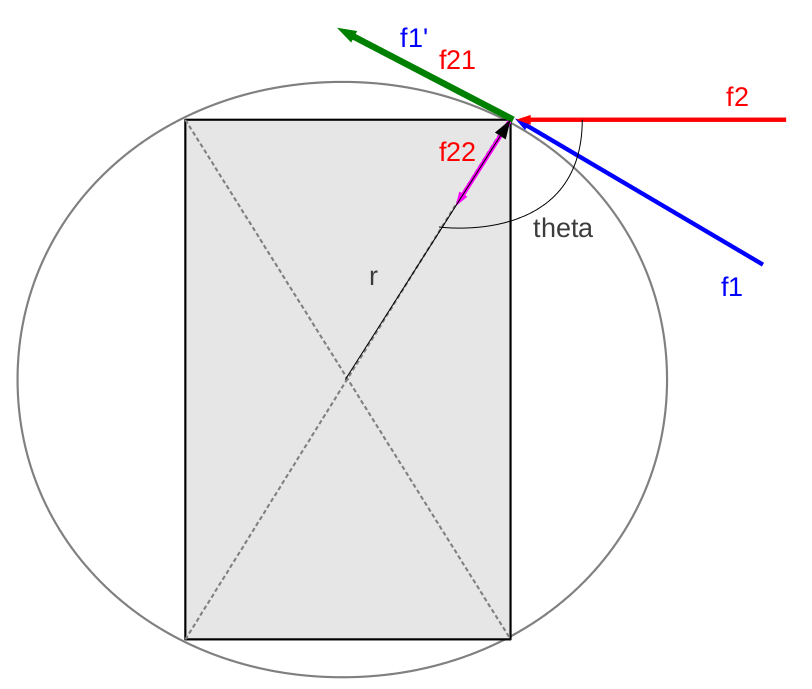
\includegraphics[width=0.5\columnwidth]{figures/rectangle-angle.png}\\


\caption[Object under the influence of two forces.]{Object under the influence of two forces. f1 shows the tangential push that will result only in the force - f1' tangential to a circle overlaid on the object (it causes only rotational movement). f2 shows the proposed pushing strategy - perpendicular to the longer edge. This push results in two forces; f21, the tangential coefficient responsible for rotation and f22, the coefficient responsible for translation. In this case the object will not only rotate but also translate in the direction of f22 force.  }
\label{fig:angles-rectangle}
\end{figure}




\begin{figure}
\centering 

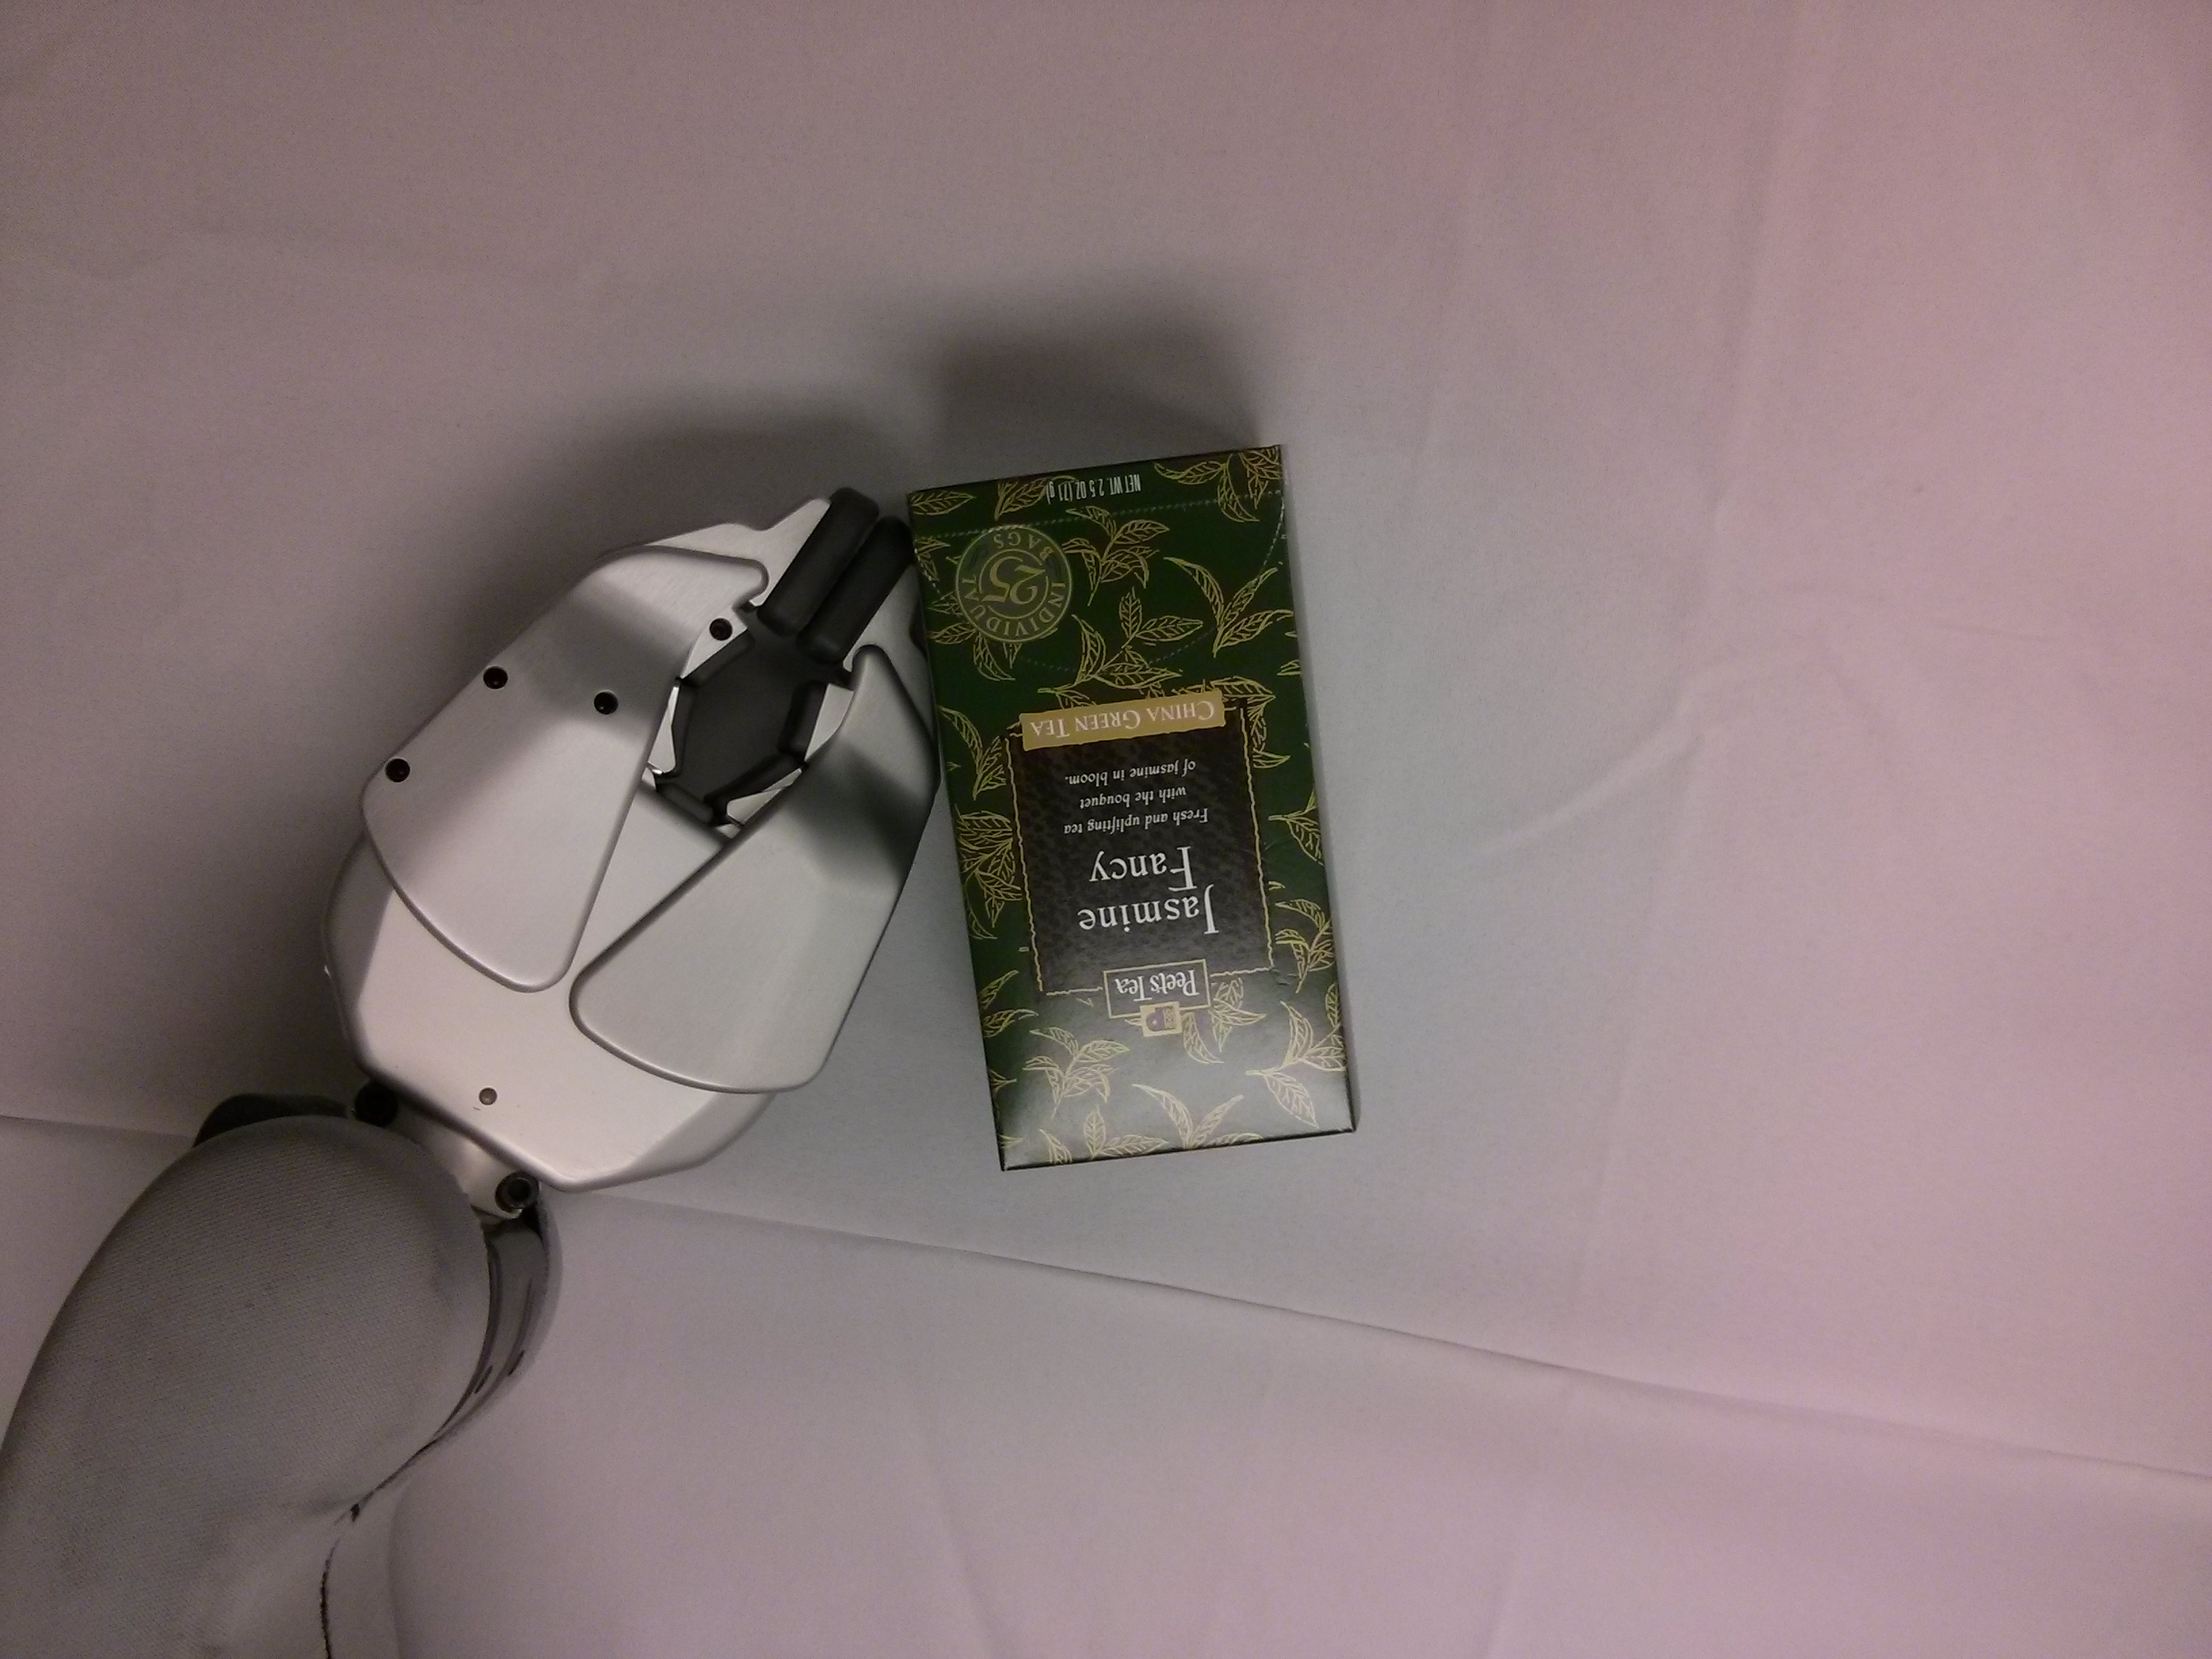
\includegraphics[width=0.4\columnwidth]{figures/peets-tangential.jpg}\\
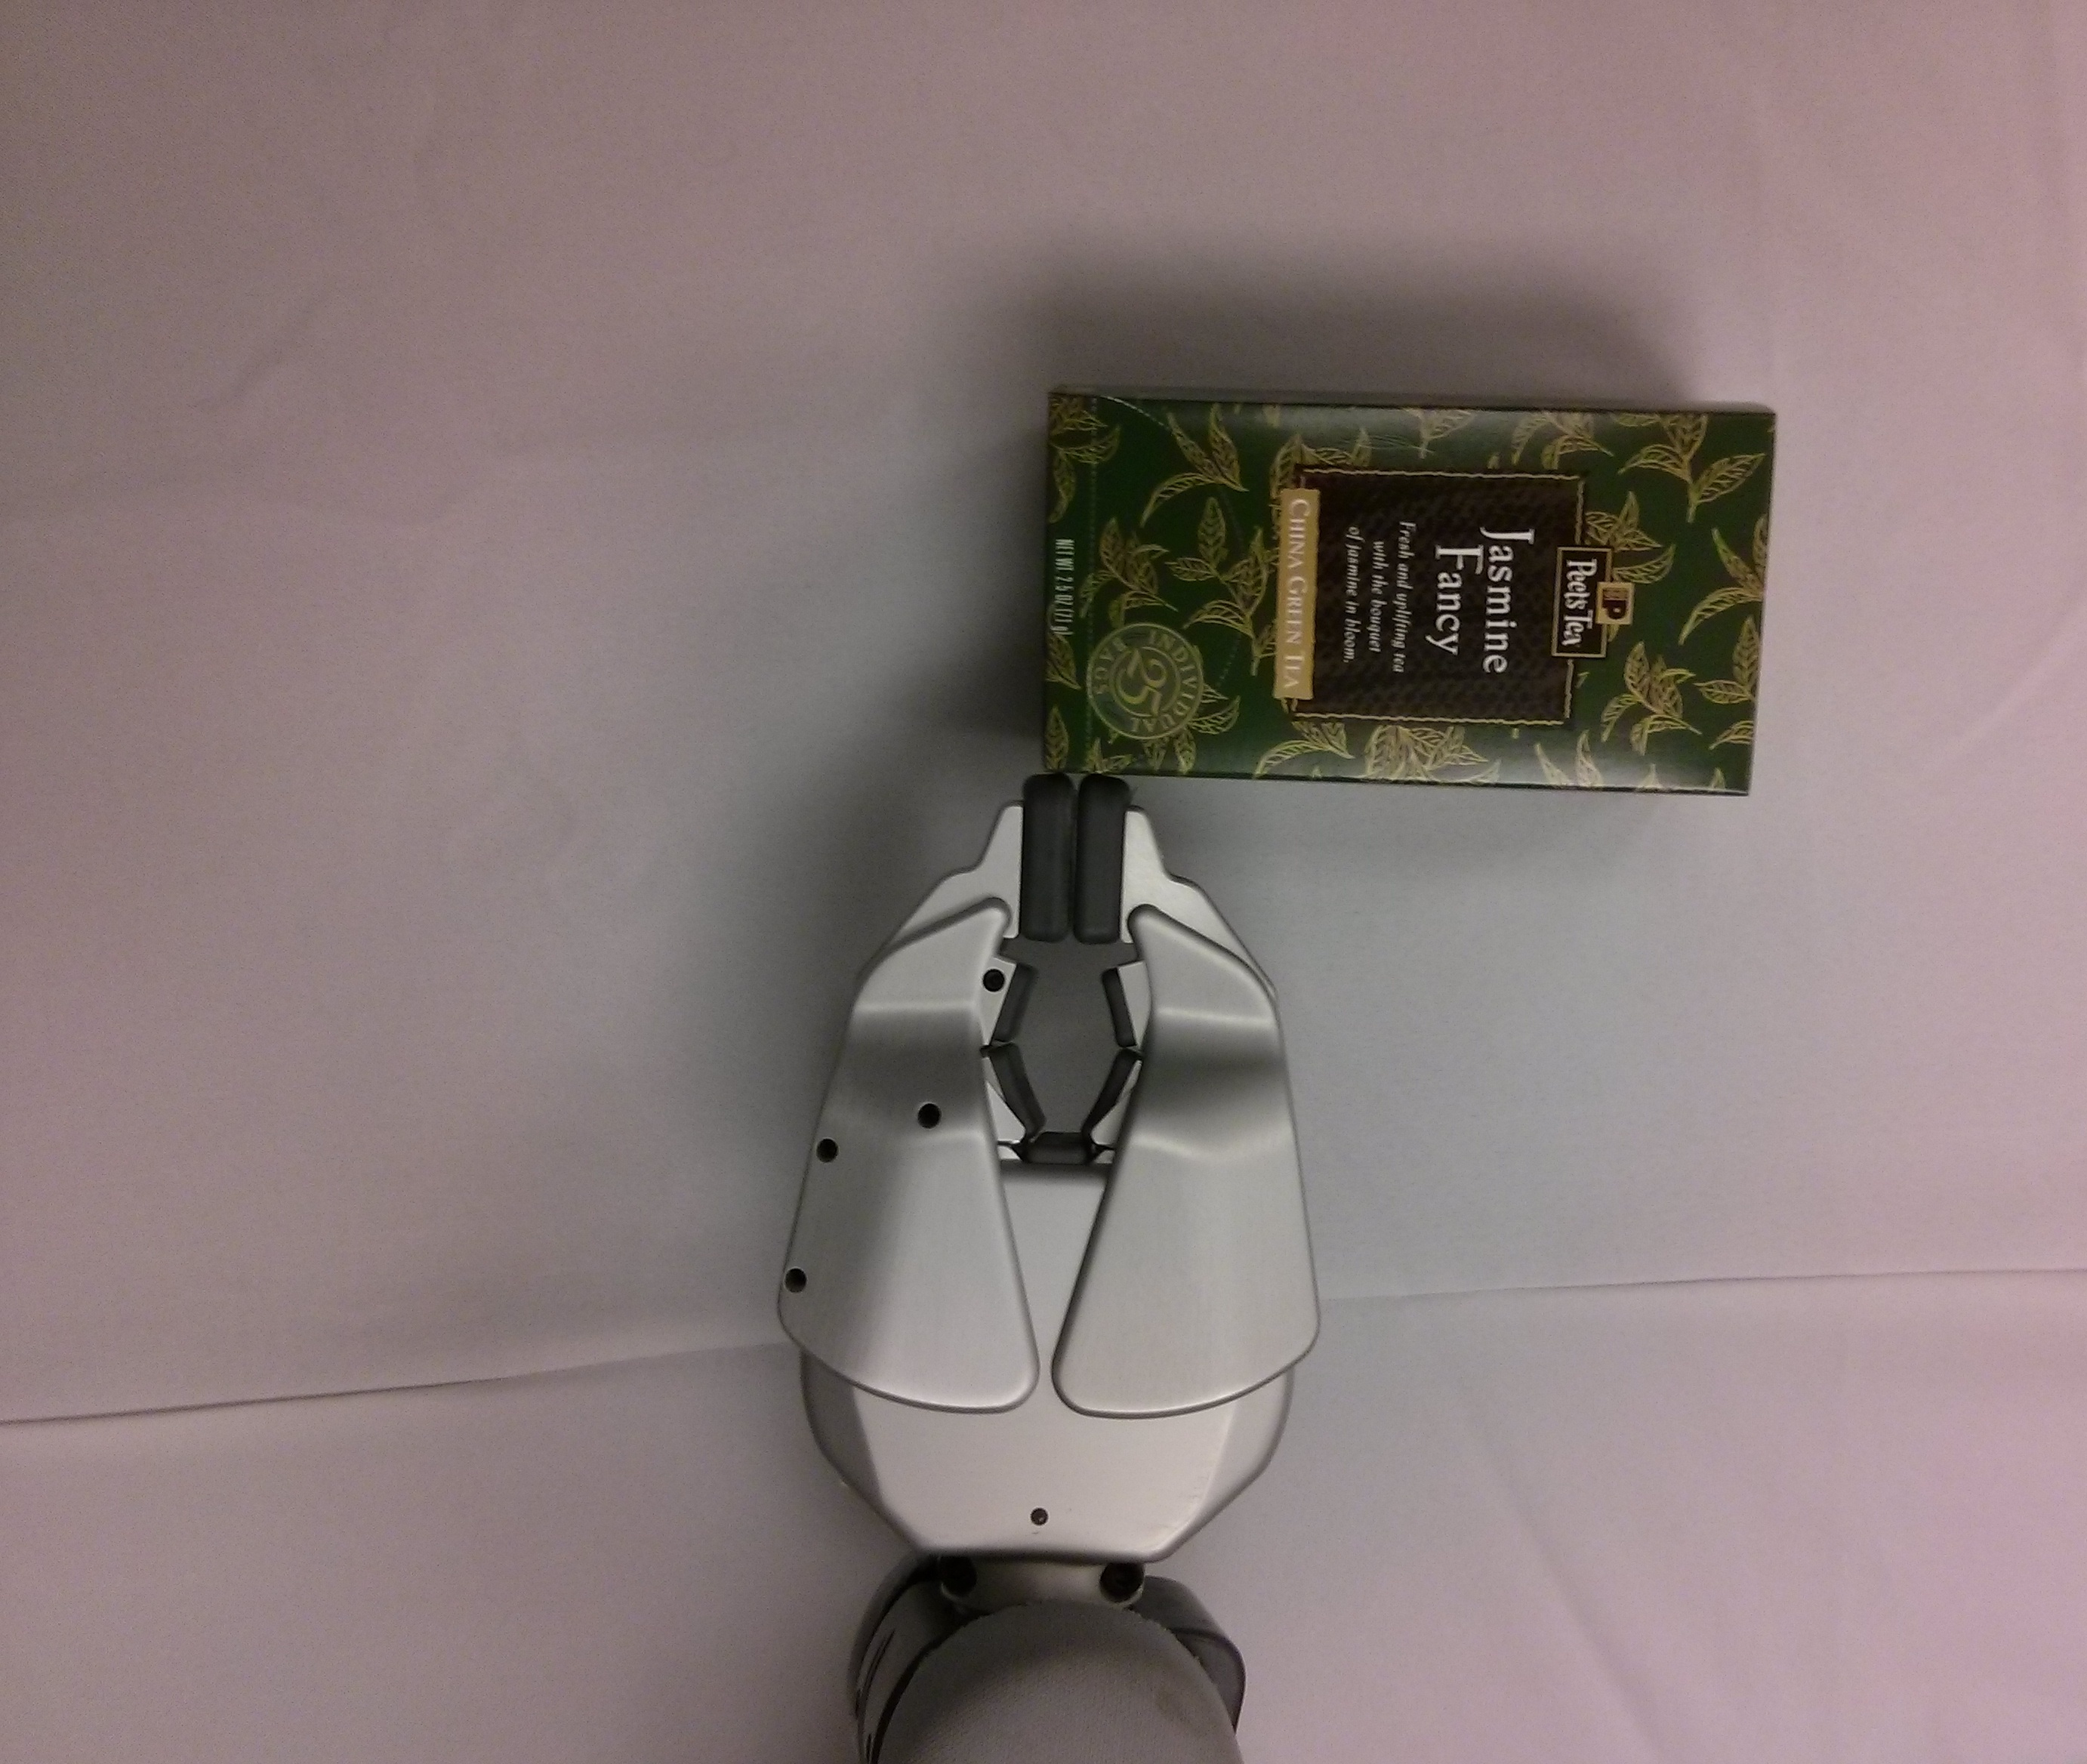
\includegraphics[width=0.4\columnwidth]{figures/peets-perpendicular.jpg}\\


\caption{Upper image - example of a tangential push. Lower image - example of a perpendicular push.}
\label{fig:tangential-example}
\end{figure}

\begin{figure}
\centering
 

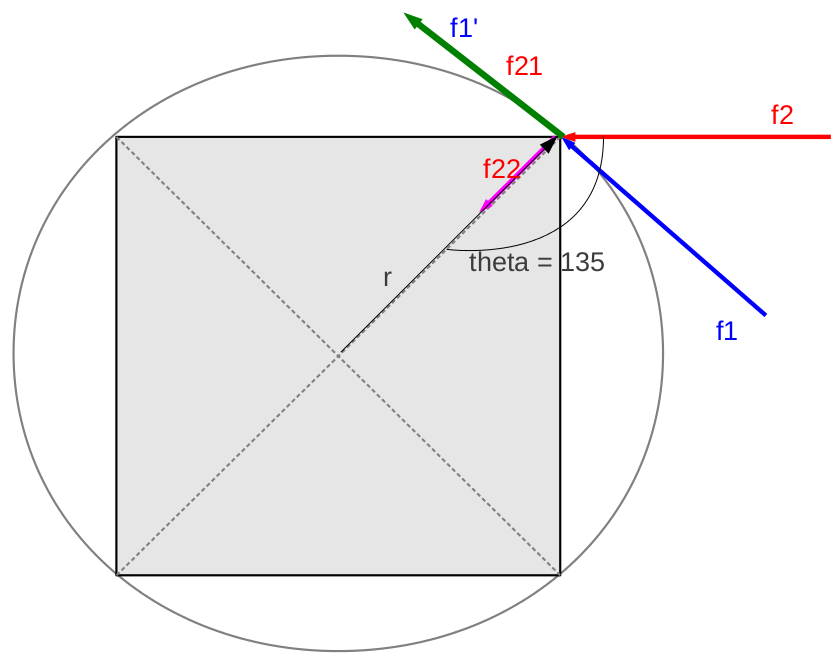
\includegraphics[width=0.5\columnwidth]{figures/square-angle.png}


\caption[Example of worst case energy loss for the proposed pushing strategy on a square object.]{Example of worst case energy loss for the proposed pushing strategy on a square object. $\theta$ is maximal in this case at $135 ^\circ$. This results in an energy loss of 29\%.  }
\label{fig:angles-square}
\end{figure}

\subsection{Rotation of Objects}
In order for the robot to rotate an object efficiently, meaning that the push results only in rotational kinematic energy, it is required to maximize the torque acting on the object. As shown in Equation \ref{eq:max-torque} the maximum torque($M$) can be obtained by maximising the ($r$ component) that the force($F$) acts on and with $sin(\theta) = 1$, where $\theta$ is the angle between the force and the radius.

\begin{equation}
M =  F \times r = F*r*sin(\theta)\\
\label{eq:max-torque}
\end{equation}

Maximizing the $r$ component results in a point that is furthest from the center of mass of the object. Since we assume uniform distribution of mass, the center of mass of the object is in its geometrical center. Hence, the best push point to rotate a rectangular object is at a corner which is furthest from the center of the rectangle.

In order to fulfil the second constraint: $sin(\theta) = 1 \to \theta = 90 ^\circ$, the robot needs to perform a tangential push. The resulting force f1 that shows this case on a rectangular object is depicted in Figure \ref{fig:angles-rectangle}. However, due to geometrical constraints of the robot's gripper it is difficult to execute a tangential push. The upper picture of Figure \ref{fig:tangential-example} shows a rectangular object with the robot's gripper in the pose for a tangential push. It can be seen that due to the size of the gripper the actual contact point between the gripper and the object is not at this corner. Another problem that occurs in this pushing strategy is that the gripper is likely to slip off the object whilst pushing it.

Due to these practical constraints of the robot gripper we propose a push perpendicular to the longer edge of the object. This push is easy to execute with the robot's gripper whilst still being able to apply rotation to the object. The lower picture of Figure \ref{fig:tangential-example} shows the resulting robot's gripper position relative to the object. However, in this case the push is not optimal in the sense that $\theta$ is not $90 ^\circ$. In order to evaluate how much push energy is lost due to translational movement we considered the worst case for this pushing strategy.  Figure \ref{fig:angles-square} shows a square object where $\theta$ is maximal and thus least optimal for the function $sin(\theta)$. From simple geometric analysis one can show that $\theta =135 ^\circ$ which results in $sin(\theta) = 0.71$.  Therefore in the worst case scenario (a square shaped object produces the worst possible $\theta$) one loses 29\% of the resulting kinematic energy to translational movement. Given the robot's configuration and the size of its gripper, this loss is considered acceptable.  It still results mostly in rotational movement of the object. 

Having developed an efficient method to rotate an object, we want to investigate the improvement this brings to the object recognition system. We claim that rotating an object significantly improves the chances of this object being recognized correctly. In addition this also makes the feature based object recognition system more computationally efficient.

\subsection{Object Recognition System}

In this section we will discuss the software architecture behind our object recognition system. The system was divided into 5 ROS packages with different responsibilities as follows:
\begin{itemize}
\item Cloud Saver - a ROS package responsible for saving an input image from the Kinect sensor to the database. A user is given a simple user interface where they can see the input image from the Kinect. It also provides functionality to save the current image together with the associated point cloud. Using this package we can create a library of images that will be later used as the database of objects that may be recognized.
\item PCL I/O - mainly responsible for reading, writing and loading different PCL data structures. It is used heavily by the Cloud Saver package.
\item Object Library - generates data for images taken by the Cloud Saver. It wraps all the data into a data structure which contains the image and the name of the object.  This data structure is easily extensible to contain other information if necessary.
\item Features - a library wrapped in a ROS package that has all the functionality to extract, describe and match different computer vision features. The features that are currently implemented in this class hold OpenCV implementations of various detector-descriptor pairs such as: SIFT, SURF~\cite{bay2006surf}, FREAK~\cite{alahi2012freak}, FAST~\cite{rosten2006machine}, BRIEF~\cite{calonder2010brief} and ORB~\cite{rublee2011orb}. It is extensively used throughout the matching phase of the system.
\item Object Matcher - the main ROS package that brings all the previous elements together. It loads all the data from the Object Library package in order to form a library of object models to be used by the object classification system. After all the objects are loaded, it calls the Features class to compute matches between input images and images in the database. At the end it outputs the score that indicates if the object was recognized and which object it is.
\end{itemize}


The packages described above form an object recognition system that enables a user to easily acquire data from a Kinect device and create a library of objects to recognize. Furthermore it then facilitates extraction, description and matching of various computer vision features on new data in order to recognize objects.




\section{Results}

\begin{figure}
%\centering 

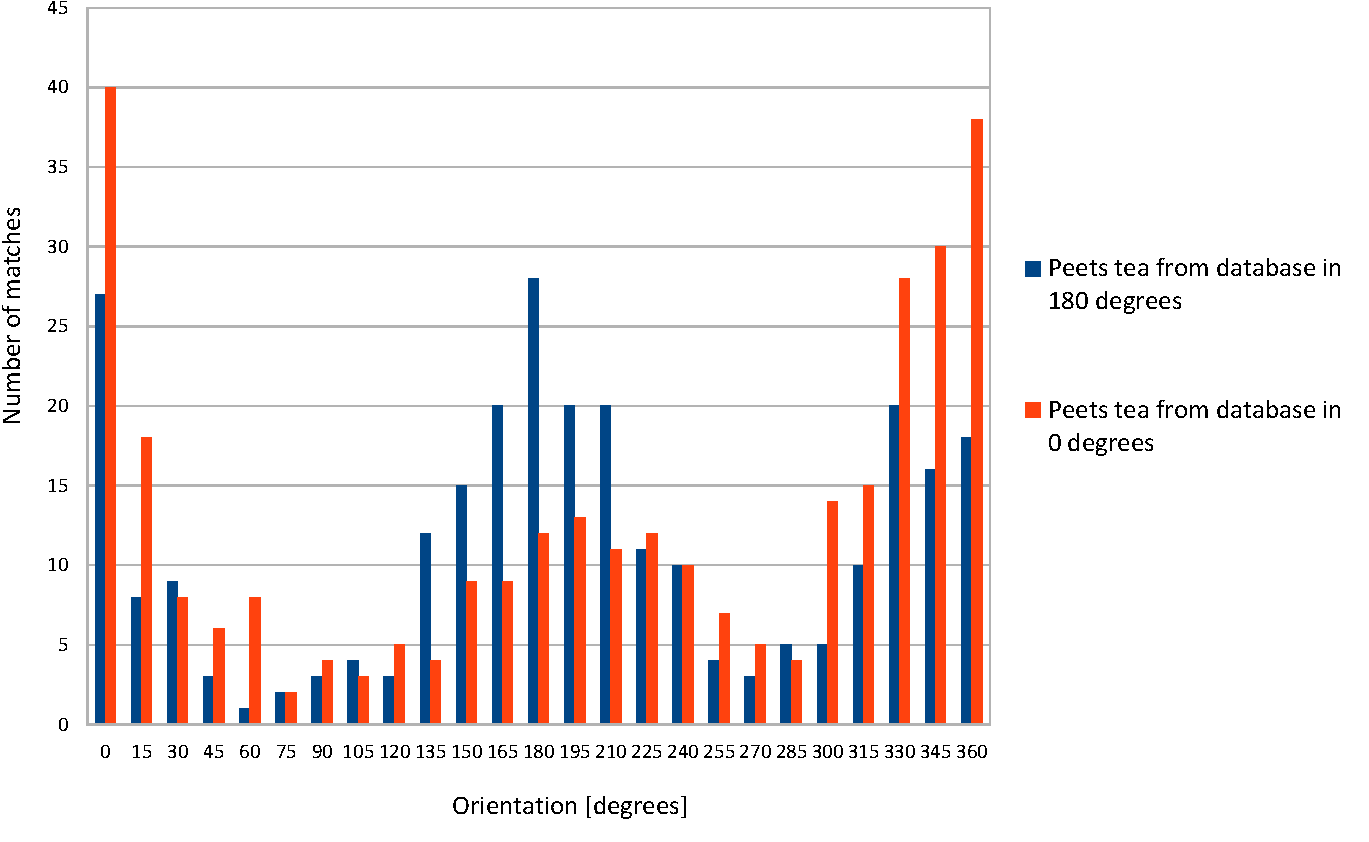
\includegraphics[width=1.3\columnwidth]{figures/print2.pdf}\\


\caption[Results of feature matching between the two images of the Peets tea box from the database and the input image of the same tea box.]{Results of feature matching between the two images of the Peets tea box from the database and the input image of the same tea box. The box was rotated 360$^\circ$ during the matching process. There are two images of the Peets tea box in the database; one rotated by 0$^\circ$ and the other one rotated by 180$^\circ$. One can note that the peaks of the number of matches are at 0$^\circ$, 180$^\circ$ and 360$^\circ$.}
\label{fig:recognition-results}
\end{figure}
%Experiments showing time with multiple templates
%Graph of different numbers of matches in relation to degrees
In this section we show how the system is evaluated on the real data. 

To test the system it was first trained with two objects: a Peets tea box and a Lipton tea box. The database maintains two images per object. The second image of each object is rotated 180$^\circ$ with respect to the orientation of the first image. For the testing phase the Peets tea box was placed in front of the Kinect. The object was then rotated 360$^\circ$ according to the movement strategy outlined in the previous section. The input images were then compared with all the images in the database. Whilst the object was being rotated the number of matches between input and database image was constantly being saved to a file. The recognition procedure was repeated three times and the results were averaged in order to reduce noise in our measurements.

Figure \ref{fig:recognition-results} shows the averaged number of matches for a given orientation of the object. The vertical axis shows the number of matches between the input image and the database image described by the respective color (see legend in Figure \ref{fig:recognition-results}). In general it can be seen that there are certain configurations where the number of matches is significantly greater. These correspond to the configurations close to the pose of the object as it occurs in the database. This shows that by rotating the object in an semi-guided manner, the recognition rate can be significantly improved. 

One can also take note that both plots in Figure \ref{fig:recognition-results} have more feature matches at the position rotated by 180$^\circ$ with respect to the image stored in the database. This is due to the symmetry of some of the features on the object used in that experiment. These features appear similar if they are rotated by 180$^\circ$, hence we obtain additional matches if the object is rotated by 180$^\circ$ with respect to the pose the algorithm was trained on.

\begin{figure}
\centering 

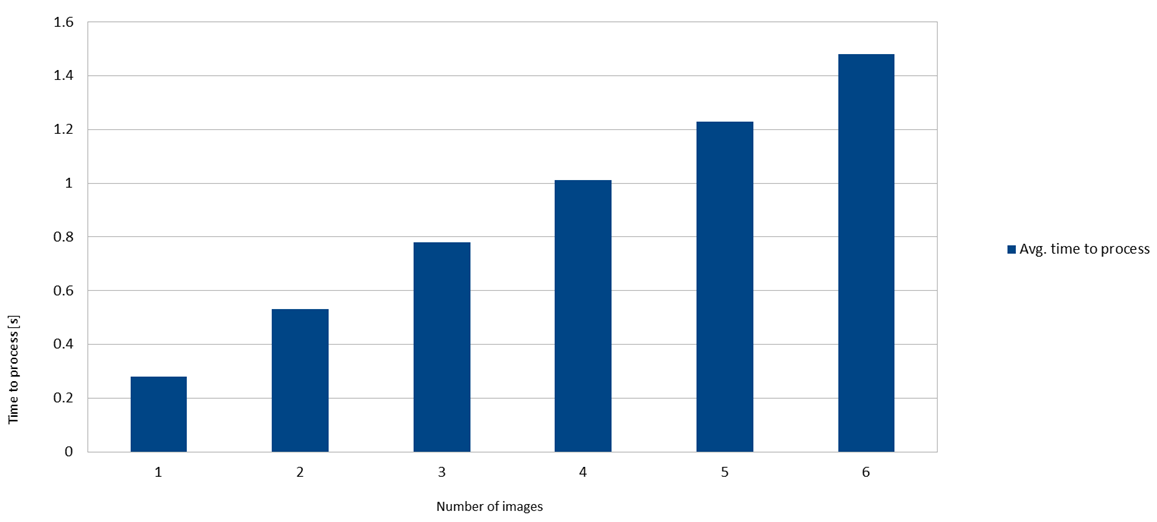
\includegraphics[width=1.2\columnwidth]{figures/thesis-time.png}\\


\caption{Processing time of the object recognition algorithm with a different number of images in the database.}
\label{fig:recognition-time}
\end{figure}

The approximate time for the system to process the data with two 640x480 resolution images during one iteration was $0.53 sec$. In one iteration we calculate matches between the input image and all the images in the database. During one iteration there were approximately 100 features found in one image. In Figure \ref{fig:recognition-time} it is apparent that the time to process a single iteration linearly scales with the number of images. Hence, the computational cost to recognize an object scales with the number of images per object in the database. By decreasing the number of images per object, we can radically decrease the computational cost of the object recognition algorithm. 
Thus, inducing motion into the scene and reducing the size of the database has a significant impact on the system performance.

In summary, one solution to pose variant features is to have a database where there are many images of different viewpoints for each object so it can always be detected regardless of orientation.  However, this means having a huge database of images.  By employing interactive perception, the same recognition rates can be obtained whilst 1) decreasing database size and 2) decreasing computational cost.  Therefore the proposed method is a valid and useful strategy for object recognition.






\section{Conclusion}
We have presented an initial implementation of a system that is able to recognize objects based on a feature matching algorithm. We have proven that inducing motion into the scene significantly improves the chance of an object being recognized correctly. In addition to that we showed that interaction with the scene allows for a smaller database which in turn reduces processing time of the system.
